\chapter{Estado de los recursos}
\label{chap:estado-recursos-CITIC-VCF}

\lettrine{C}{on} el fin de contextualizar los recursos que se utilizarán en este trabajo, en este capítulo se expone la situación actual de toda la infraestructura en lo relacionado al software que está en funcionamiento, a los recursos físicos de los que se compone, y al estado actual de las herramientas que rodean a dichos recursos.

\begin{section}{Infraestructura}
La infraestructura física donde se planea desplegar el servicio de virtualización, se encuentra localizada en el edificio del CITIC de la UDC, dentro de un rack alojado en su Centro de Proceso de Datos (CPD) \cite{citicUDC}. 
\begin{subsection}{Cómputo}
    La forman 5 nodos \textit{Lenovo NeXtScale nx360 M5} cada uno con dos procesadores Intel Xeon E5-2650, 128 GB de memoria RAM y una tarjeta gráfica Tesla M60,  y 3 nodos \textit{Dell EMC PowerEdge R740} cada uno con dos procesadores Xeon Gold 6146, 384 GB de memoria RAM y una tarjeta gráfica Tesla P40. Todos ellos aportan flexibilidad en cuanto a la escalabilidad de la infraestructura y ofrecen gran rendimiento de cómputo.
\end{subsection}
\begin{subsection}{Almacenamiento}
    El almacenamiento está colocado físicamente en la misma ubicación que los hosts pero en su abstracción lógica este es independiente y está separado de cada nodo. Está conformado por 13 discos duros SSD de 3.84 TB de capacidad, obteniendo así una cantidad total de casi 50 TB pero la capacidad útil es de 34 TB ya que se utiliza la configuración de almacenamiento RAID 5[Pal. \ref{itm:raid5}] para aporta mayor  integridad de los datos, mayor tolerancia a fallos y mayor ancho de banda. Los discos duros están colocados en una misma cabina donde forman un \textit{pool} de almacenamiento que se divide en cinco LUNs (\textit{Logical Storage Unit})[Pal. \ref{itm:lun}] de 2 TB cada una, representadas en el software de virtualización como cinco \textit{datastores} y que emplean el sistema de archivos VMFS propio de la compañía VMware y el cual optimiza el almacenamiento de máquinas virtuales.
    La configuración y gestión de este sistema se tiene que realizar al nivel de la capa física, por lo tanto si se quiere hacer un despliegue en el sistema de virtualización con una configuración de almacenamiento diferente a la existente, como por ejemplo un sistema RAID con diferentes características, sería necesario modificar la configuración del sistema físico pudiendo generar un gran coste de tiempo. Esto no permite ajustar de forma precisa y rápida las configuraciones que se necesitan para realizar despliegues sobre la infraestructura.
\end{subsection}

\begin{subsection}{Red}
    El sistema de almacenamiento forma una SAN, para ello las conexiones que se implementan entre los nodos y las cabinas donde se encuentran los discos duros son de tipo 10 Gbit. Para soportar esta conexión, cada cabina incorpora dos controladores SFP+[Pal. \ref{itm:sfp}]. Además, las cabinas de almacenamiento incorporan otros dos puertos de 1 Gbit para la administración de los discos. En esta estructura se utilizan los protocolos de red Ethernet y iSCSI. Finalmente, para mantener la disponibilidad del acceso al sistema de almacenamiento y las comunicaciones entre los nodos, cada uno de ellos se conecta a dos switches \textit{trunk} estableciendo rutas redundantes.
    Igual que con el sistema de almacenamiento, si se requieren realizar modificaciones sobre la red para adaptarse a los requisitos de un determinado despliegue habría que hacerlas directamente sobre la red física. Esto puede generar problemas en la conectividad del entorno a parte de generar gran coste de tiempo.

\end{subsection}

\end{section}

\begin{section}{Software}
    \label{subsec:softwareinstalado}
    Actualmente, el software desplegado sobre la infraestructura está formado por los productos de la compañía VMware, uno de los principales proveedores de software de virtualización, siendo \textbf{VMware vSphere}, versión 6.7, el principal componente ya que se utiliza para virtualizar parte de la infraestructura física y proporcionar las herramientas necesarias para gestionarla, sus principales componentes internos se describen a continuación.
    \begin{figure}[h]
        \centering
        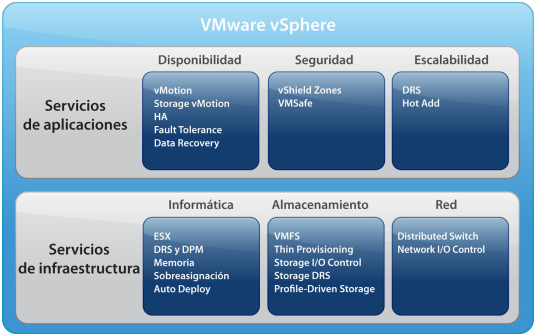
\includegraphics[width=0.75\textwidth]{imaxes/cap2recursos/contentVSphere}
        \caption{Componentes de VMware vSphere\cite{fotovSphere}}
        \label{fig:vSphere-components}
      \end{figure}
    En cada nodo físico está instalado el \textbf{hipervisor ESXi} de tipo baremetal. Sobre los nodos corre el servicio \textbf{VMware vCenter Server} que actúa como centro de administración de todas las máquinas virtuales (VMs) y nodos que forman la infraestructura y, además, contiene una instancia embebida de \textbf{Platform Services Controller} (PSC) punto que centraliza el acceso a distintos servicios como APIs de VMware vCenter Server, servidor de licencias o el servicio de autenticación \textbf{vCenter Single Sign-On}, este último se utiliza para gestionar la autenticación de los usuarios registrados en VMware vCenter Server. El acceso e interfaz de VMware vCenter Server se realiza a través de la página \textbf{vSphere Web Client} donde el usuario puede autenticarse y gestionar las VMs y nodos que forman el entorno y el resto de servicios de VMware vSphere. Además, incorpora \textbf{vSphere Update Manager} que permite gestionar las actualizaciones de software de los componentes de VMware vSphere. Para administrar las conexiones de las VMs, vSphere utiliza \textbf{vSphere Distributed Switch} (vDS), un switch virtual que gestiona el tráfico de cada VM permitiendo indicar que interfaces físicas de cada nodo físico, configurar sus puertos, establecer políticas y crear subredes de forma centralizada. Finalmente, existen varios servicios de gran importancia que se encargan de mantener la disponibilidad de las VMs desplegadas sobre la infraestructura:
    
    \begin{itemize}
        \item \textbf{vMotion} y \textbf{Storage vMotion}: el primero se encarga de migrar VMs de un nodo a otro de forma transparente y sin detener su ejecución, permitiendo planificar las migraciones. El segundo servicio se encarga de migrar los discos y configuración de una VM de un \textit{datastore} a otro sin interrumpir el servicio.
        
        \item \textbf{vSphere High Availability} (HA): En caso de que una VM deje de estar activa, este servicio intenta encenderla de forma automática en otro nodo del entorno. A diferencia de vMotion, este solo actúa en caso de que la VM o el nodo donde se encuentra la VM sufra un fallo y esta pase a estar no disponible. 
        
        \item \textbf{vSphere Distributed Resource Scheduler} (DRS), \textbf{vSphere Distributed Power Management} (DPM) y \textbf{Sotrage DRS}: vSphere DRS genera recomendaciones sobre donde se debería desplegar una máquina virtual durante su creación, utiliza vMotion para migrar las VMs y así maximizar el rendimiento o para manterner la VM activa durante tareas de mantenimiento en un nodo. vSphere DPM se encarga de gestionar el consumo de energía de cada host según el rendimiento actual. Sotrage DRS se encarga de balancear la carga de almacenamiento y las operaciones de lectura y escritura entre los \textit{datastores} disponibles.
        
        \item \textbf{vSphere Fault Tolerance}: gestiona una copia de todos los archivos y discos de cada VM sincronizada con los archivos originales. Este servicio usado con vSphere HA y vSphere DRS proporciona recuperación ante fallos automática y disponibilidad continua de las VMs, sin perdida de datos y sin pérdida de las conexiones establecidas. En caso de que una VM deje de estar disponible esta se reinicia en un nodo diferente. Este servicio está orientado a proteger aquellas tareas que requieren un alto rendimiento o que son críticas.
    \end{itemize}
\end{section}

\begin{figure}[hp]
    \centering
    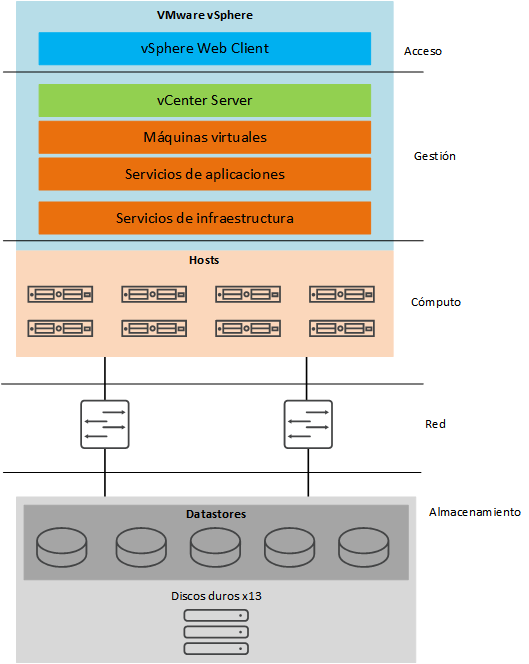
\includegraphics[width=0.6\textwidth]{imaxes/cap2recursos/recursosReal.png}
    \caption{Componentes físicos y software que forman la infraestructura actual.}
    \label{fig:infrastructure-components-production}
\end{figure}
\FloatBarrier

\begin{section}{Estado de la tecnología}
Con el desarrollo de las tecnologías web y la comercialización por parte de grandes empresas de su infraestructura los servicios \textit{Infrastructure as a Service} (IaaS) han ganado una popularidad considerable, con ello también se han desarrollado herramientas software dedicadas a la gestión infraestructura para la implementación de sistemas Cloud Computing. Algunas de estos servicios son VMware Cloud Foundation (creado en 2011), OpenStack (creado en 2010) o Apache CloudStack (creado en 2012). Estas herramientas construyen una infraestructura virtual sobre un conjunto de recursos físicos estandarizados que permite separar la administración de la capa física de la capa virtual, para simplificar y automatizar la gestión y escalabilidad de los recursos físicos y virtuales. Esto persigue reducir costes de gestión de la infraestructura y aumentar la disponibilidad del servicio, es decir, aumentar la eficiencia de la infraestructura física.

Si bien en el mercado existen varias alternativas que se pueden desplegar\footnote{OpenStack y Apache CloudStack entre otras.} sobre la infraestructura existente, finalmente, para cumplir los objetivos de este proyecto se ha escogido el producto \textbf{VMware Cloud Foundation} (VCF) ya que se integra perfectamente con los componentes de VMware ya instalados en la infraestructura y, por lo tanto, su mantenimiento a largo plazo es más sencillo. Desplegar un producto de una compañía diferente podría producir problemas de compatibilidad entre versiones a largo plazo, a pesar de que este se pueda integrar con el software VMware vSphere. Utilizando los productos de un mismo proveedor se asegura el soporte de las diferentes versiones del software instalado y la obtención del máximo rendimiento de cada componente.
Para poder usar este software es necesaria la adquisición de licencias, estas se organizan por componente y por número de hosts sobre los que se va a instalar el producto. Aunque tienen un coste elevado, este producto aporta grandes beneficios en cuanto a la gestión del SDDC.
\begin{subsection}{VMware Cloud Foundation}

    Esta solución de VMware virtualiza todas las capas de la infraestructura combinando cuatro de sus productos. Utiliza \textbf{VMware vSphere} para virtualizar y gestionar el cómputo, \textbf{VMware vSAN} para virtualizar y gestionar el almacenamiento, \textbf{VMware NSX-T} para la virtualización y gestión de la red, y \textbf{VMware vRealize} para gestionar las operaciones de la infraestructura virtual como el aprovisionamiento de recursos o la gestión de \textit{logs} centralizada. Todos juntos, estos servicios convierten el CPD en un \textit{Software Defined Datacenter} (SDDC), un entorno donde existe una infraestructura física que se abstrae en una capa virtual para separar la gestión de ambas y poder modificar la infraestructura virtual según las necesidades de los usuarios sin necesidad de modificar la configuración de la infraestructura física. Gracias a esa estructura obtiene las siguientes características:
\begin{itemize}

    \item \textbf{Servicios software con integración nativa}: ofrece un conjunto de servicios software para el almacenamiento, red, seguridad y gestión de la cloud. Estos servicios se integran de forma nativa con la infraestructura minimizando las tareas de configuración y administración.

    \item \textbf{Escalabilidad y elasticidad de los recursos}: la capacidad de la infraestructura se puede modificar de forma sencilla gracias a la automatización del ciclo de vida de todos los elementos y al desacople entre las dos capas (la física y la virtual).

    \item \textbf{Supervisión de los recursos}: ofrece supervisión de los recursos con reconocimiento de aplicaciones y solución de problemas, permitiendo conocer todos los eventos que tienen lugar en la infraestructura. También permite establecer políticas de seguridad en cuanto al acceso a los recursos y la red.

    \item \textbf{Aprovisionamiento automatizado}: permite la otención de recursos de forma automática incluyendo servicios de red, almacenamiento y cómputo. Los componentes de la infraestructura virtualizada se encargan de la reserva de los recursos y de todas las operaciones necesarias para llevarla acabo.

    \item \textbf{Ciclo de vida automatizado}: automatiza las operaciones previas, iniciales y posterios de los recursos de la plataforma para simplificar y coordinar su gestión. En estas tareas se incluye desde el despliegue de la plataforma y su implementación, el aprovisionamiento de nuevos recursos físicos y la instalación de actualizaciones para cada componente software.

\end{itemize}
\begin{figure}[h!]
    \centering
    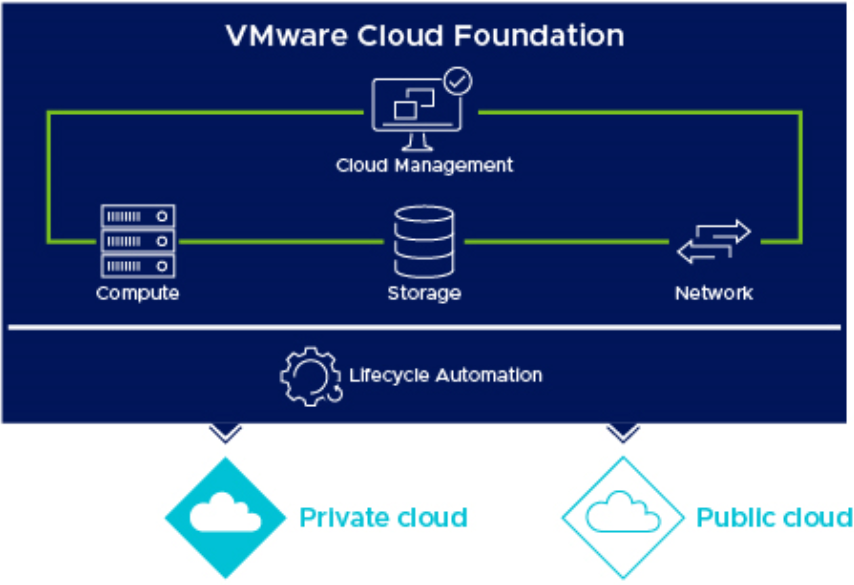
\includegraphics[width=0.6\textwidth]{imaxes/cap2recursos/overviewCF.png}
            \caption{Resumen partes de VMare Cloud Foundation.}
    \label{fig:Cloud-Foundation-Overview}
    \end{figure}
    \FloatBarrier
    \begin{figure}[h]
        \centering
        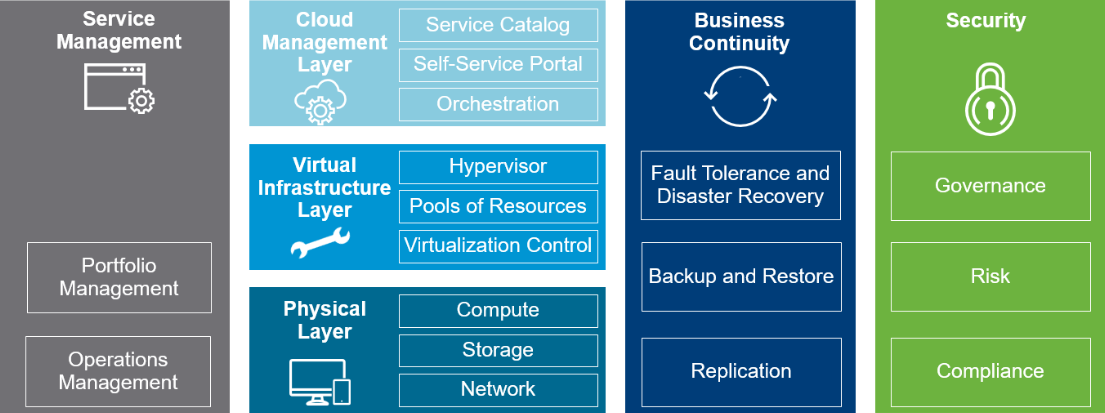
\includegraphics[width=0.8\textwidth]{imaxes/cap2recursos/SDDCoverview.png}
        \caption{Elementos de un SDDC gestionado con VMware Cloud Foundation.}
        \label{fig:layers-Sddc}
    \end{figure}
    \FloatBarrier
\end{subsection}

\begin{subsection}{Componentes de VMware Cloud Foundation}
\label{subsubsect:cfcomponents}

Ya se ha visto que VCF está formado por cuatro productos principales de VMware. En este apartado se describirán las características de esos cuatro componentes más el servicio que los coordina\footnote{Las características del componente VMware vSphere son las mismas que las descritas en el punto \ref*{subsec:softwareinstalado}}. Se utilizará la versión 4.0 de VMware Cloud Foundation lo cual implica que se implementarán las versiones\cite{componentesCloudFound} 4.0 de SDDC Manager, 7.0.0 de VMware vSphere, 7.0.0 de VMware vSAN, 3.0 de VMware NSX-T y 8.1 de VMware vRealize Suite.
\begin{figure}[h]
    \centering
        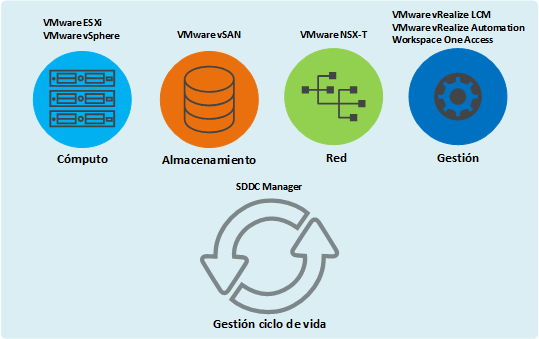
\includegraphics[width=0.6\textwidth]{imaxes/VCF-componentes/ComponentesVCF.png}
        \caption{Partes de un SDDC y componentes de VCF que las implementan.}
        \label{fig:componentes-funciones-VCF}
    \end{figure}
    \FloatBarrier
\begin{subsubsection}{SDDC Manager}
    SDDC Manager se encarga de gestionar el ciclo de vida de todos los componentes de VCF, esto incluye el despliegue de cada uno, su configuración y la obtención e instalación de actualizaciones. Centraliza la gestión de las licencias y certificados de cada componente y administra el aprovisionamiento de nuevos recursos físicos para el SDDC y los ya existentes.
\end{subsubsection}

\begin{subsubsection}{VMware vSAN}
    VMware vSAN virtualiza el almacenamiento del SDDC. Permite gestionar de forma centralizada desde la interfaz de vSphere Web Client el sistema de almacenamiento sin necesidad de tener que modificar la configuración física, como es el caso de las LUNs de la infraestructura actual. Trata todos los recursos de almacenamiento como un único elmento denominado \textit{datastore} sobre el cual se pueden establecer políticas incluso a nivel de VM lo cual aporta gran flexibilidad. El acceso por parte de cada nodo al \textit{datastore} se realiza con el protocolo IP a través de una subred dedicada al servicio. Con VMware vSAN, el \textit{datastore} esta formado por discos de almacenamiento se organizan en grupos ligados a un nodo (un máximo de cinco grupos por nodo). Los grupos pueden tener configuración \textit{Hybrid} que combinia discos HDD y SDD, o configuración \textit{All-Flash} que solo utiliza SSD y por lo tanto tiene mayor rendimiento. Dentro de cada grupo existe un disco de caché y al menos un disco de capacidad donde se almacenan los datos persistentes\cite{operacionesVSAN}. En el modo \textit{All-Flash}\footnote{Solo se describe el modo \textit{All-Flash} porque es la configuración recomendada por VMware.} la operación de lectura se realiza directamente sobre los discos de capacidad y la operación de escritura se hace sobre el disco caché que posteriormente escribe los datos en el disco de capacidad.
    
    \begin{figure}[h]
    \centering
        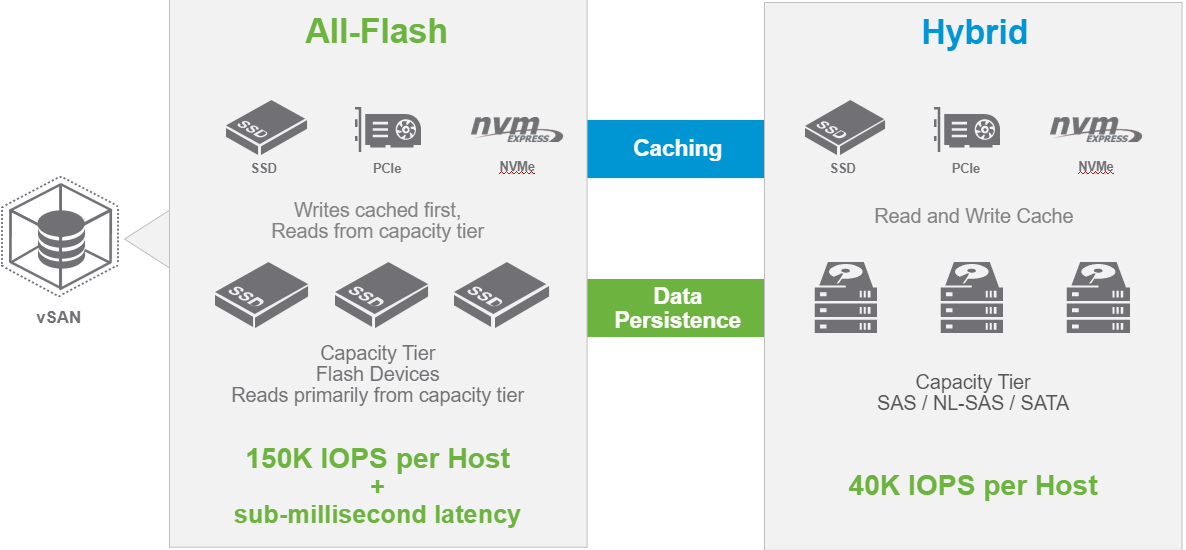
\includegraphics[width=0.6\textwidth]{imaxes/cap2recursos/rendimientoVSAN.png}
        \caption{Configuración \textit{All-Flash} y configuración \textit{Hybrid} en vSAN}
        \label{fig:performance-Hybrid-AllFlash-vSAN}
    \end{figure}
    \FloatBarrier
\end{subsubsection}

\begin{subsubsection}{VMware NSX-T}
    VMware NSX-T virtualiza la red del SDDC. Abstrae los componentes físicos de la red para generar una red virtual desacoplada de la infraestructura física que se puede configurar sin modificar la red física, para ello aporta servicios de red virtualizados y la posibilidad de crear y extender subredes. Internamente está formado por varias instancias de \textbf{NSX-T Manager Appliance} que a su vez se compone de \textit{NSX-T Manager} y \textbf{NSX-T Controller}. El primero es el punto de acceso a la configuración de VMware NSX-T y el que almacena y transmite la configuración establecida, el segundo controla las redes y servicios virtuales aportando la información y configuración necesarias para que gestionen el tráfico correctamente y obteniendo estadísticas sobre este. El control del tráfico y la monitorización de las conexiones se hace desde el componente \textbf{Transport Node} (TN) con la información que recibe de las instancias de NSX-T Controller. Existen dos tipos de TNs, \textbf{Hypervisor Transport Node} que son nodos con ESXi instalado y que están configurados para correr los servicios de VMware NSX-T, y \textbf{NSX-T Edge Node} que se trata de una \textit{appliance} instalada en una VM o sobre un nodo físico para proveer un conjunto de servicios de red centralizados para las redes virtuales de VMware NSX-T.
    \begin{figure}[h!]
        \centering
            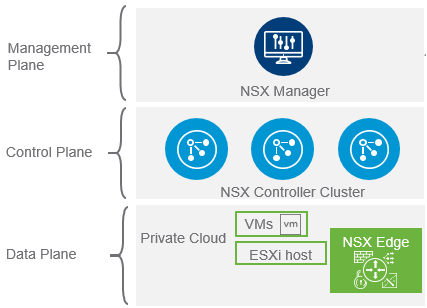
\includegraphics[width=0.6\textwidth]{imaxes/VCF-componentes/nsx-t-layers.png}
            \caption{Componentes de VMware NSX-T y capas en las que se dividen}
            \label{fig:nsx-t-components}
        \end{figure}
        \FloatBarrier
\end{subsubsection}

\begin{subsubsection}{VMware vRealize Suite}
    VMware vRealize Suite agrupa un conjunto de productos que si bien no son obligatorios para desplegar VCF, aportan funcionalidades extra que completan la formación del SDDC. Los productos que se utilizarán en este proyecto son \textbf{vRealize Suite Lifecycle Manager} dedicado a gestionar el desliegue, actualizaciones, certificados y licencias de los productos que forman VMware vRealize, \textbf{Workspace One Access} dedicado a gestionar los usuarios y ser el punto de acceso centralizado de las aplicaciones de VMware vRealize y, finalmente, \textbf{vRealize Automation} el cual permite a los usuarios del SDDC diseñar y aprovisionar un conjunto de recursos de la infraestructura según sus necesidades y de forma automatizada mientras el administrador puede limitar la cantidad de recursos que se consumen.
\end{subsubsection}

\end{subsection}

\end{section}
